\documentclass[12pt,a4paper]{article}
\usepackage[utf8]{vietnam}
\usepackage{amsmath,amssymb}
\usepackage{tabularx}
\usepackage{tikz}
\usepackage{xcolor}
\usepackage[top=0.6cm, bottom=0.6cm, left=0.6cm, right=0.6cm]{geometry}
\usepackage[dethi]{ex_test}

\SAOPTN{widthSA=2.6,heightSA=0.62}
\setlength{\parskip}{0pt}

% Dong ke cham mo chuan viet tay
\newcommand{\dongke}[1]{%
  \begingroup%
  \setlength{\parskip}{0pt}%
  \baselineskip=18.5pt%
  \vspace{1.0mm}%
  \foreach \i in {1,...,#1}{%
    \noindent{\color{gray!60}\dotfill}\par%
  }%
  \vspace{0.6mm}%
  \endgroup%
}

% Dinh nghia o bai tap tu luan trong bang
\newcommand{\oBaiTap}[3][5]{%
  \vspace{1.0mm}%
  \noindent\textbf{#2} #3\par%
  \dongke{#1}%
}

\begin{document}
\pagestyle{empty}
% =============================================================================
% ========================= MA DE 101 - MAT TRUOC (TRANG 1/2) =============
% =============================================================================
\noindent
\begin{tabularx}{\linewidth}{|X|c|}
\hline
\textbf{PHIẾU KIỂM TRA ĐỊNH KỲ TOÁN 9 - TUẦN 12 - BUỔI 01} & \textbf{Mã đề: 101 - Trang 1/2} \\
\hline
\end{tabularx}

\vspace{1.0mm}

\noindent
\begin{tabularx}{\linewidth}{|p{3.2cm}|X|}
\hline
\centering\textbf{ĐIỂM SỐ} & \centering\textbf{LỜI NHẬN XÉT CỦA THẦY CÔ} \tabularnewline
\hline
\rule{0pt}{1.8cm} & \tabularnewline
\hline
\end{tabularx}

\vspace{1.2mm}
\noindent\textbf{Câu 1 (0,25 điểm).} Cho điểm $A$ ngoài $(O; 5\text{ cm})$, tiếp tuyến $AB$. $OA = 13\text{ cm} \implies AB =$ \shortans{12\text{ cm}}\par\vspace{0.8mm}
\noindent\textbf{Câu 2 (0,25 điểm).} Cho $AB, AC$ là hai tiếp tuyến của $(O)$, $\widehat{BOC} = 120^\circ \implies \widehat{BAC} =$ \shortans{60^\circ}\par\vspace{0.8mm}
\noindent\textbf{Câu 3 (0,25 điểm).} Khoảng cách từ tâm $O$ đến tiếp tuyến của $(O; R)$ bằng: \shortans{R}\par\vspace{0.8mm}
\noindent\textbf{Câu 4 (0,25 điểm).} Giá trị biểu thức $\sqrt{(4 - \sqrt{17})^2} =$ \shortans{\sqrt{17} - 4}\par\vspace{0.8mm}
\noindent\textbf{Câu 5 (0,25 điểm).} Điều kiện xác định của $\dfrac{1}{\sqrt{x - 3}}$ là: \shortans{x > 3}\par\vspace{0.8mm}
\noindent\textbf{Câu 6 (0,25 điểm).} Tính giá trị: $\sqrt{45} - \sqrt{20} + \sqrt{5} =$ \shortans{2\sqrt{5}}\par\vspace{0.8mm}
\noindent\textbf{Câu 7 (0,25 điểm).} Nghiệm của hệ $\begin{cases} 2x + y = 7 \\ x - y = 2 \end{cases}$ là $(x; y) =$ \shortans{(3; 1)}\par\vspace{0.8mm}
\noindent\textbf{Câu 8 (0,25 điểm).} $\Delta$ vuông cạnh $6\text{ cm}, 8\text{ cm}$ có đường cao là: \shortans{4{,}8\text{ cm}}\par\vspace{0.8mm}
\noindent\textbf{Câu 9 (0,25 điểm).} Hai tiếp tuyến tại $B, C$ của $(O)$ cắt nhau tại $A$. Khi đó $OA \perp$ \shortans{BC}\par\vspace{0.8mm}
\noindent\textbf{Câu 10 (0,25 điểm).} Bánh xe có $d = 50\text{ cm}$, lăn $10$ vòng đi được: \shortans{5\pi\text{ m}}\par\vspace{0.8mm}
\vspace{0.6mm}
\noindent\textbf{Câu 11 (2,5 điểm).}
\vspace{0.6mm}

\noindent
\begin{tabularx}{\linewidth}{|X|X|}
\hline
\oBaiTap[19]{a)}{Giải hệ phương trình:\par\vspace{1.0mm}$\begin{cases} 2x + y = 5 \\ 3x - 2y = 4 \end{cases}$} & 
\oBaiTap[19]{b)}{Cho biểu thức $P = \left(\dfrac{\sqrt{x}}{\sqrt{x} + 2} + \dfrac{4\sqrt{x}}{x - 4}\right) : \dfrac{\sqrt{x} + 2}{x - 4}$ ($x \ge 0;\, x \neq 4$).\par Rút gọn $P$ và tính giá trị của $P$ tại $x = 9$.} \\
\hline
\end{tabularx}

\newpage
% =============================================================================
% ========================= MA DE 101 - MAT SAU (TRANG 2/2) ==============
% =============================================================================
\noindent
\begin{tabularx}{\linewidth}{|X|c|}
\hline
\textbf{TOÁN 9 - TUẦN 12 - BUỔI 01} & \textbf{Mã đề: 101 - Trang 2/2} \\
\hline
\end{tabularx}

\vspace{3.0mm}

\noindent
\begin{tabularx}{\linewidth}{|X|}
\hline
\vspace{0.5mm}
\textbf{Câu 12 (2,5 điểm).} Một ô tô và một xe máy cùng khởi hành một lúc từ hai địa điểm $A$ và $B$ cách nhau $180\text{ km}$, đi ngược chiều nhau và gặp nhau sau $2$ giờ. Biết mỗi giờ ô tô đi nhanh hơn xe máy $10\text{ km}$. Tính vận tốc của mỗi xe.\par
\vspace{0.4mm}
\noindent\textit{Bài giải:}\dongke{16}
\\ \hline
\end{tabularx}

\vspace{7.5mm}

\noindent
\begin{tabularx}{\linewidth}{|X|}
\hline
\vspace{0.5mm}
\begin{minipage}[t]{0.56\linewidth}
\vspace{0pt}
\textbf{Câu 13 (2,5 điểm).} Cho đường tròn $(O; R)$ và điểm $A$ nằm bên ngoài đường tròn. Từ $A$ kẻ hai tiếp tuyến $AB, AC$ với đường tròn $(O)$ ($B, C$ là các tiếp điểm). Gọi $H$ là giao điểm của $OA$ và $BC$.\par\vspace{0.4mm}
\textbf{a)} Chứng minh bốn điểm $A, B, O, C$ cùng thuộc một đường tròn.\par\vspace{0.4mm}
\textbf{b)} Chứng minh $OA \perp BC$ tại $H$ và $\triangle OHB \backsim \triangle OBA$, từ đó suy ra $OH \cdot OA = R^2$.
\end{minipage}\hspace{4mm}
\begin{minipage}[t]{0.41\linewidth}
\vspace{0pt}\raggedright
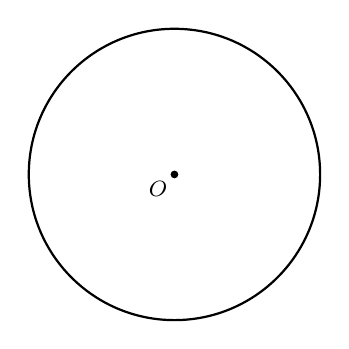
\begin{tikzpicture}[>=stealth, line join=round, line cap=round, font=\footnotesize]
  \coordinate (O) at (1.9, 0);
  \draw[thick] (O) circle (1.85cm);
  \fill (O) circle (1.4pt) node[below left=-1pt] {$O$};
\end{tikzpicture}
\end{minipage}\par
\vspace{0.4mm}
\noindent\textit{Bài giải:}\dongke{13}
\\ \hline
\end{tabularx}

\newpage
% =============================================================================
% ========================= MA DE 102 - MAT TRUOC (TRANG 1/2) =============
% =============================================================================
\noindent
\begin{tabularx}{\linewidth}{|X|c|}
\hline
\textbf{PHIẾU KIỂM TRA ĐỊNH KỲ TOÁN 9 - TUẦN 12 - BUỔI 01} & \textbf{Mã đề: 102 - Trang 1/2} \\
\hline
\end{tabularx}

\vspace{1.0mm}

\noindent
\begin{tabularx}{\linewidth}{|p{3.2cm}|X|}
\hline
\centering\textbf{ĐIỂM SỐ} & \centering\textbf{LỜI NHẬN XÉT CỦA THẦY CÔ} \tabularnewline
\hline
\rule{0pt}{1.8cm} & \tabularnewline
\hline
\end{tabularx}

\vspace{1.2mm}
\noindent\textbf{Câu 1 (0,25 điểm).} Cho điểm $A$ ngoài $(O; 6\text{ cm})$, tiếp tuyến $AB$. $OA = 10\text{ cm} \implies AB =$ \shortans{8\text{ cm}}\par\vspace{0.8mm}
\noindent\textbf{Câu 2 (0,25 điểm).} Cho $AB, AC$ là hai tiếp tuyến của $(O)$, $\widehat{BOC} = 110^\circ \implies \widehat{BAC} =$ \shortans{70^\circ}\par\vspace{0.8mm}
\noindent\textbf{Câu 3 (0,25 điểm).} Đường thẳng vuông góc bán kính tại tiếp điểm là: \shortans{Tiếp tuyến}\par\vspace{0.8mm}
\noindent\textbf{Câu 4 (0,25 điểm).} Giá trị biểu thức $\sqrt{(3 - \sqrt{11})^2} =$ \shortans{\sqrt{11} - 3}\par\vspace{0.8mm}
\noindent\textbf{Câu 5 (0,25 điểm).} Điều kiện xác định của $\dfrac{1}{\sqrt{x - 5}}$ là: \shortans{x > 5}\par\vspace{0.8mm}
\noindent\textbf{Câu 6 (0,25 điểm).} Tính giá trị: $\sqrt{48} - \sqrt{27} + \sqrt{3} =$ \shortans{2\sqrt{3}}\par\vspace{0.8mm}
\noindent\textbf{Câu 7 (0,25 điểm).} Nghiệm của hệ $\begin{cases} x + 2y = 7 \\ x - y = 1 \end{cases}$ là $(x; y) =$ \shortans{(3; 2)}\par\vspace{0.8mm}
\noindent\textbf{Câu 8 (0,25 điểm).} $\Delta$ vuông cạnh $9\text{ cm}, 12\text{ cm}$ có đường cao là: \shortans{7{,}2\text{ cm}}\par\vspace{0.8mm}
\noindent\textbf{Câu 9 (0,25 điểm).} Hai tiếp tuyến tại $B, C$ của $(O)$ cắt nhau tại $A$. Khi đó $AB =$ \shortans{AC}\par\vspace{0.8mm}
\noindent\textbf{Câu 10 (0,25 điểm).} Bánh xe có $d = 60\text{ cm}$, lăn $10$ vòng đi được: \shortans{6\pi\text{ m}}\par\vspace{0.8mm}
\vspace{0.6mm}
\noindent\textbf{Câu 11 (2,5 điểm).}
\vspace{0.6mm}

\noindent
\begin{tabularx}{\linewidth}{|X|X|}
\hline
\oBaiTap[19]{a)}{Giải hệ phương trình:\par\vspace{1.0mm}$\begin{cases} 3x + y = 7 \\ 2x - 3y = 1 \end{cases}$} & 
\oBaiTap[19]{b)}{Cho biểu thức $P = \left(\dfrac{\sqrt{x}}{\sqrt{x} + 3} + \dfrac{6\sqrt{x}}{x - 9}\right) : \dfrac{\sqrt{x} + 3}{x - 9}$ ($x \ge 0;\, x \neq 9$).\par Rút gọn $P$ và tính giá trị của $P$ tại $x = 16$.} \\
\hline
\end{tabularx}

\newpage
% =============================================================================
% ========================= MA DE 102 - MAT SAU (TRANG 2/2) ==============
% =============================================================================
\noindent
\begin{tabularx}{\linewidth}{|X|c|}
\hline
\textbf{TOÁN 9 - TUẦN 12 - BUỔI 01} & \textbf{Mã đề: 102 - Trang 2/2} \\
\hline
\end{tabularx}

\vspace{3.0mm}

\noindent
\begin{tabularx}{\linewidth}{|X|}
\hline
\vspace{0.5mm}
\textbf{Câu 12 (2,5 điểm).} Một ô tô và một xe máy cùng khởi hành một lúc từ hai địa điểm $A$ và $B$ cách nhau $150\text{ km}$, đi ngược chiều nhau và gặp nhau sau $1{,}5$ giờ. Biết mỗi giờ ô tô đi nhanh hơn xe máy $20\text{ km}$. Tính vận tốc của mỗi xe.\par
\vspace{0.4mm}
\noindent\textit{Bài giải:}\dongke{16}
\\ \hline
\end{tabularx}

\vspace{7.5mm}

\noindent
\begin{tabularx}{\linewidth}{|X|}
\hline
\vspace{0.5mm}
\begin{minipage}[t]{0.56\linewidth}
\vspace{0pt}
\textbf{Câu 13 (2,5 điểm).} Cho đường tròn $(O; R)$ và điểm $A$ nằm bên ngoài đường tròn. Từ $A$ kẻ hai tiếp tuyến $AB, AC$ với đường tròn $(O)$ ($B, C$ là các tiếp điểm). Gọi $H$ là giao điểm của $OA$ và $BC$.\par\vspace{0.4mm}
\textbf{a)} Chứng minh bốn điểm $A, B, O, C$ cùng thuộc một đường tròn.\par\vspace{0.4mm}
\textbf{b)} Chứng minh $OA \perp BC$ tại $H$ và $\triangle OHB \backsim \triangle OBA$, từ đó suy ra $OH \cdot OA = R^2$.
\end{minipage}\hspace{4mm}
\begin{minipage}[t]{0.41\linewidth}
\vspace{0pt}\raggedright
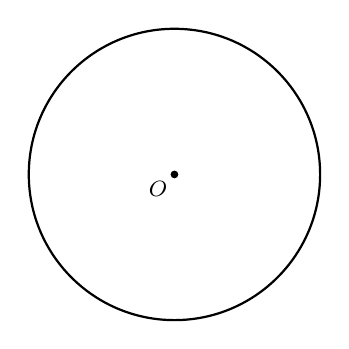
\begin{tikzpicture}[>=stealth, line join=round, line cap=round, font=\footnotesize]
  \coordinate (O) at (1.9, 0);
  \draw[thick] (O) circle (1.85cm);
  \fill (O) circle (1.4pt) node[below left=-1pt] {$O$};
\end{tikzpicture}
\end{minipage}\par
\vspace{0.4mm}
\noindent\textit{Bài giải:}\dongke{13}
\\ \hline
\end{tabularx}

\newpage
% =============================================================================
% ========================= MA DE 103 - MAT TRUOC (TRANG 1/2) =============
% =============================================================================
\noindent
\begin{tabularx}{\linewidth}{|X|c|}
\hline
\textbf{PHIẾU KIỂM TRA ĐỊNH KỲ TOÁN 9 - TUẦN 12 - BUỔI 01} & \textbf{Mã đề: 103 - Trang 1/2} \\
\hline
\end{tabularx}

\vspace{1.0mm}

\noindent
\begin{tabularx}{\linewidth}{|p{3.2cm}|X|}
\hline
\centering\textbf{ĐIỂM SỐ} & \centering\textbf{LỜI NHẬN XÉT CỦA THẦY CÔ} \tabularnewline
\hline
\rule{0pt}{1.8cm} & \tabularnewline
\hline
\end{tabularx}

\vspace{1.2mm}
\noindent\textbf{Câu 1 (0,25 điểm).} Cho điểm $A$ ngoài $(O; 8\text{ cm})$, tiếp tuyến $AB$. $OA = 17\text{ cm} \implies AB =$ \shortans{15\text{ cm}}\par\vspace{0.8mm}
\noindent\textbf{Câu 2 (0,25 điểm).} Cho $AB, AC$ là hai tiếp tuyến của $(O)$, $\widehat{BAC} = 50^\circ \implies \widehat{BOC} =$ \shortans{130^\circ}\par\vspace{0.8mm}
\noindent\textbf{Câu 3 (0,25 điểm).} Số tiếp tuyến kẻ từ một điểm ngoài đường tròn tới $(O)$ là: \shortans{2}\par\vspace{0.8mm}
\noindent\textbf{Câu 4 (0,25 điểm).} Giá trị biểu thức $\sqrt{(5 - \sqrt{26})^2} =$ \shortans{\sqrt{26} - 5}\par\vspace{0.8mm}
\noindent\textbf{Câu 5 (0,25 điểm).} Điều kiện xác định của $\dfrac{1}{\sqrt{x - 4}}$ là: \shortans{x > 4}\par\vspace{0.8mm}
\noindent\textbf{Câu 6 (0,25 điểm).} Tính giá trị: $\sqrt{32} - \sqrt{18} + \sqrt{2} =$ \shortans{2\sqrt{2}}\par\vspace{0.8mm}
\noindent\textbf{Câu 7 (0,25 điểm).} Nghiệm của hệ $\begin{cases} 3x - y = 8 \\ x + y = 4 \end{cases}$ là $(x; y) =$ \shortans{(3; 1)}\par\vspace{0.8mm}
\noindent\textbf{Câu 8 (0,25 điểm).} $\Delta$ vuông cạnh $5\text{ cm}, 12\text{ cm}$ có cạnh huyền là: \shortans{13\text{ cm}}\par\vspace{0.8mm}
\noindent\textbf{Câu 9 (0,25 điểm).} Hai tiếp tuyến tại $B, C$ của $(O)$ cắt ở $A$. Phân giác $\widehat{BAC}$ là: \shortans{AO}\par\vspace{0.8mm}
\noindent\textbf{Câu 10 (0,25 điểm).} Bánh xe có $d = 70\text{ cm}$, lăn $10$ vòng đi được: \shortans{7\pi\text{ m}}\par\vspace{0.8mm}
\vspace{0.6mm}
\noindent\textbf{Câu 11 (2,5 điểm).}
\vspace{0.6mm}

\noindent
\begin{tabularx}{\linewidth}{|X|X|}
\hline
\oBaiTap[19]{a)}{Giải hệ phương trình:\par\vspace{1.0mm}$\begin{cases} 2x - y = 3 \\ x + 2y = 4 \end{cases}$} & 
\oBaiTap[19]{b)}{Cho biểu thức $P = \left(\dfrac{\sqrt{x}}{\sqrt{x} - 1} - \dfrac{2\sqrt{x}}{x - 1}\right) : \dfrac{\sqrt{x} - 1}{x - 1}$ ($x \ge 0;\, x \neq 1$).\par Rút gọn $P$ và tính giá trị của $P$ tại $x = 25$.} \\
\hline
\end{tabularx}

\newpage
% =============================================================================
% ========================= MA DE 103 - MAT SAU (TRANG 2/2) ==============
% =============================================================================
\noindent
\begin{tabularx}{\linewidth}{|X|c|}
\hline
\textbf{TOÁN 9 - TUẦN 12 - BUỔI 01} & \textbf{Mã đề: 103 - Trang 2/2} \\
\hline
\end{tabularx}

\vspace{3.0mm}

\noindent
\begin{tabularx}{\linewidth}{|X|}
\hline
\vspace{0.5mm}
\textbf{Câu 12 (2,5 điểm).} Một ô tô và một xe máy cùng khởi hành một lúc từ hai địa điểm $A$ và $B$ cách nhau $210\text{ km}$, đi ngược chiều nhau và gặp nhau sau $2$ giờ. Biết mỗi giờ ô tô đi nhanh hơn xe máy $15\text{ km}$. Tính vận tốc của mỗi xe.\par
\vspace{0.4mm}
\noindent\textit{Bài giải:}\dongke{16}
\\ \hline
\end{tabularx}

\vspace{7.5mm}

\noindent
\begin{tabularx}{\linewidth}{|X|}
\hline
\vspace{0.5mm}
\begin{minipage}[t]{0.56\linewidth}
\vspace{0pt}
\textbf{Câu 13 (2,5 điểm).} Cho đường tròn $(O; R)$ và điểm $A$ nằm bên ngoài đường tròn. Từ $A$ kẻ hai tiếp tuyến $AB, AC$ với đường tròn $(O)$ ($B, C$ là các tiếp điểm). Gọi $H$ là giao điểm của $OA$ và $BC$.\par\vspace{0.4mm}
\textbf{a)} Chứng minh bốn điểm $A, B, O, C$ cùng thuộc một đường tròn.\par\vspace{0.4mm}
\textbf{b)} Chứng minh $OA \perp BC$ tại $H$ và $\triangle OHB \backsim \triangle OBA$, từ đó suy ra $OH \cdot OA = R^2$.
\end{minipage}\hspace{4mm}
\begin{minipage}[t]{0.41\linewidth}
\vspace{0pt}\raggedright
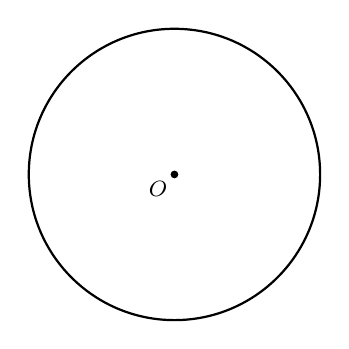
\begin{tikzpicture}[>=stealth, line join=round, line cap=round, font=\footnotesize]
  \coordinate (O) at (1.9, 0);
  \draw[thick] (O) circle (1.85cm);
  \fill (O) circle (1.4pt) node[below left=-1pt] {$O$};
\end{tikzpicture}
\end{minipage}\par
\vspace{0.4mm}
\noindent\textit{Bài giải:}\dongke{13}
\\ \hline
\end{tabularx}

\newpage
% =============================================================================
% ========================= MA DE 104 - MAT TRUOC (TRANG 1/2) =============
% =============================================================================
\noindent
\begin{tabularx}{\linewidth}{|X|c|}
\hline
\textbf{PHIẾU KIỂM TRA ĐỊNH KỲ TOÁN 9 - TUẦN 12 - BUỔI 01} & \textbf{Mã đề: 104 - Trang 1/2} \\
\hline
\end{tabularx}

\vspace{1.0mm}

\noindent
\begin{tabularx}{\linewidth}{|p{3.2cm}|X|}
\hline
\centering\textbf{ĐIỂM SỐ} & \centering\textbf{LỜI NHẬN XÉT CỦA THẦY CÔ} \tabularnewline
\hline
\rule{0pt}{1.8cm} & \tabularnewline
\hline
\end{tabularx}

\vspace{1.2mm}
\noindent\textbf{Câu 1 (0,25 điểm).} Cho điểm $A$ ngoài $(O; 9\text{ cm})$, tiếp tuyến $AB$. $OA = 15\text{ cm} \implies AB =$ \shortans{12\text{ cm}}\par\vspace{0.8mm}
\noindent\textbf{Câu 2 (0,25 điểm).} Cho $AB, AC$ là hai tiếp tuyến của $(O)$, $\widehat{BAC} = 70^\circ \implies \widehat{BOC} =$ \shortans{110^\circ}\par\vspace{0.8mm}
\noindent\textbf{Câu 3 (0,25 điểm).} Cho $(O; 5\text{ cm})$. Khoảng cách từ $O$ đến tiếp tuyến là: \shortans{5\text{ cm}}\par\vspace{0.8mm}
\noindent\textbf{Câu 4 (0,25 điểm).} Giá trị biểu thức $\sqrt{(2 - \sqrt{7})^2} =$ \shortans{\sqrt{7} - 2}\par\vspace{0.8mm}
\noindent\textbf{Câu 5 (0,25 điểm).} Điều kiện xác định của $\dfrac{1}{\sqrt{x - 6}}$ là: \shortans{x > 6}\par\vspace{0.8mm}
\noindent\textbf{Câu 6 (0,25 điểm).} Tính giá trị: $\sqrt{75} - \sqrt{12} + \sqrt{27} =$ \shortans{6\sqrt{3}}\par\vspace{0.8mm}
\noindent\textbf{Câu 7 (0,25 điểm).} Nghiệm của hệ $\begin{cases} 2x - y = 5 \\ x + y = 4 \end{cases}$ là $(x; y) =$ \shortans{(3; 1)}\par\vspace{0.8mm}
\noindent\textbf{Câu 8 (0,25 điểm).} $\Delta$ vuông cạnh $3\text{ cm}, 4\text{ cm}$ có đường cao là: \shortans{2{,}4\text{ cm}}\par\vspace{0.8mm}
\noindent\textbf{Câu 9 (0,25 điểm).} Hai tiếp tuyến tại $B, C$ của $(O)$ cắt ở $A$. Phân giác $\widehat{BOC}$ là: \shortans{OA}\par\vspace{0.8mm}
\noindent\textbf{Câu 10 (0,25 điểm).} Bánh xe có $d = 80\text{ cm}$, lăn $10$ vòng đi được: \shortans{8\pi\text{ m}}\par\vspace{0.8mm}
\vspace{0.6mm}
\noindent\textbf{Câu 11 (2,5 điểm).}
\vspace{0.6mm}

\noindent
\begin{tabularx}{\linewidth}{|X|X|}
\hline
\oBaiTap[19]{a)}{Giải hệ phương trình:\par\vspace{1.0mm}$\begin{cases} x + 2y = 5 \\ 3x - y = 1 \end{cases}$} & 
\oBaiTap[19]{b)}{Cho biểu thức $P = \left(\dfrac{\sqrt{x}}{\sqrt{x} - 2} - \dfrac{4\sqrt{x}}{x - 4}\right) : \dfrac{\sqrt{x} - 2}{x - 4}$ ($x \ge 0;\, x \neq 4$).\par Rút gọn $P$ và tính giá trị của $P$ tại $x = 9$.} \\
\hline
\end{tabularx}

\newpage
% =============================================================================
% ========================= MA DE 104 - MAT SAU (TRANG 2/2) ==============
% =============================================================================
\noindent
\begin{tabularx}{\linewidth}{|X|c|}
\hline
\textbf{TOÁN 9 - TUẦN 12 - BUỔI 01} & \textbf{Mã đề: 104 - Trang 2/2} \\
\hline
\end{tabularx}

\vspace{3.0mm}

\noindent
\begin{tabularx}{\linewidth}{|X|}
\hline
\vspace{0.5mm}
\textbf{Câu 12 (2,5 điểm).} Một ô tô và một xe máy cùng khởi hành một lúc từ hai địa điểm $A$ và $B$ cách nhau $160\text{ km}$, đi ngược chiều nhau và gặp nhau sau $2$ giờ. Biết mỗi giờ ô tô đi nhanh hơn xe máy $20\text{ km}$. Tính vận tốc của mỗi xe.\par
\vspace{0.4mm}
\noindent\textit{Bài giải:}\dongke{16}
\\ \hline
\end{tabularx}

\vspace{7.5mm}

\noindent
\begin{tabularx}{\linewidth}{|X|}
\hline
\vspace{0.5mm}
\begin{minipage}[t]{0.56\linewidth}
\vspace{0pt}
\textbf{Câu 13 (2,5 điểm).} Cho đường tròn $(O; R)$ và điểm $A$ nằm bên ngoài đường tròn. Từ $A$ kẻ hai tiếp tuyến $AB, AC$ với đường tròn $(O)$ ($B, C$ là các tiếp điểm). Gọi $H$ là giao điểm của $OA$ và $BC$.\par\vspace{0.4mm}
\textbf{a)} Chứng minh bốn điểm $A, B, O, C$ cùng thuộc một đường tròn.\par\vspace{0.4mm}
\textbf{b)} Chứng minh $OA \perp BC$ tại $H$ và $\triangle OHB \backsim \triangle OBA$, từ đó suy ra $OH \cdot OA = R^2$.
\end{minipage}\hspace{4mm}
\begin{minipage}[t]{0.41\linewidth}
\vspace{0pt}\raggedright
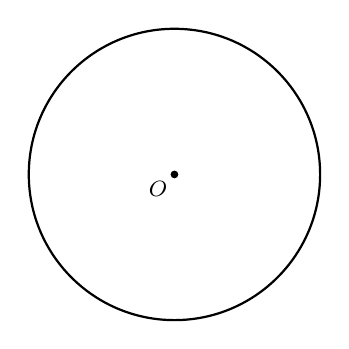
\begin{tikzpicture}[>=stealth, line join=round, line cap=round, font=\footnotesize]
  \coordinate (O) at (1.9, 0);
  \draw[thick] (O) circle (1.85cm);
  \fill (O) circle (1.4pt) node[below left=-1pt] {$O$};
\end{tikzpicture}
\end{minipage}\par
\vspace{0.4mm}
\noindent\textit{Bài giải:}\dongke{13}
\\ \hline
\end{tabularx}
\end{document}
